% \begin{frame}
%   \frametitle{Motivation - Cryptography}
%   \begin{itemize}
%     \item Is ubiquitous
%     \item Often Hardware-focused
%     \item This project has focused on implementing a variety of algorithms instead of nitpicking one algorithm.
%   \end{itemize}
% \end{frame}

\begin{frame}
  \frametitle{Motivation - Why use FPGAs?}
  \begin{minipage}[b]{0.45\textwidth}
    \begin{itemize}
    \item Architecture
    \item Configurable not only in computation but also in interface
    \item Often fast as the overhead from generality is ommitted
    \item Often lower power consumption than CPU's
    \item Difficult to program (Xilinx Vivado {\DejaSans 😩})
    \end{itemize}
  \end{minipage}
  \vspace{30px}
  \begin{minipage}[b]{0.50\textwidth}
    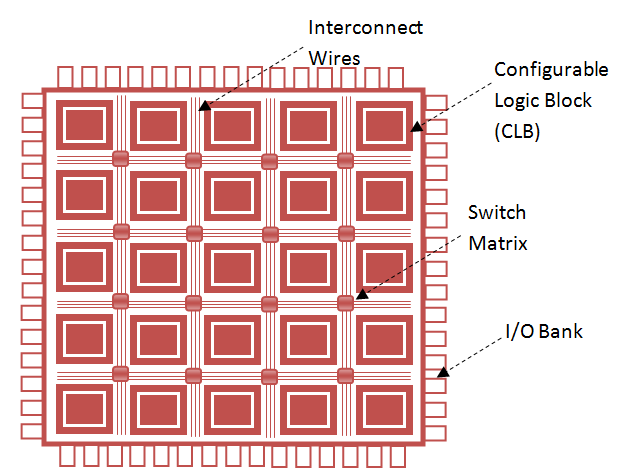
\includegraphics[width=5cm]{FPGA_Arch}
    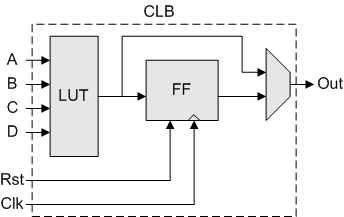
\includegraphics[width=4cm]{CLB}
  \end{minipage}
\end{frame}

\begin{frame}
  \frametitle{Motivation - Why use SME?}
  \begin{itemize}
  \item Synchronous Message Exchange
  \item High-level software programming for Hardware
  \item Based on Communicating Sequential Processes
%%     %% \begin{itemize}
%%     %% \item A program consists of a set of named processes
%%     %% \item Each process runs concurrently with no form of sharing with other processes
%%     %% \item Concurrent processes can communicate using message passing
%%     %% \end{itemize}
  \item Consists of; a \verb~simple process~, and a \verb~clocked process~ with input and output busses, and an \verb~onTick()~ function. Together with a \verb~simulation process~ for testing
  \end{itemize}
\end{frame}
